\documentclass[tikz,convert={outfile=\jobname.svg}]{standalone}
\usetikzlibrary{automata, arrows.meta, positioning}
\begin{document} 
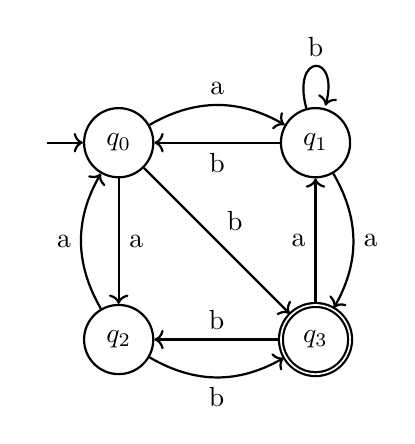
\begin{tikzpicture}[
    thick,
    node distance={25mm},
    auto
]

\node[state, initial, initial text = {}] (q0) {$q_0$}; 
\node[state] (q1) [right of=q0] {$q_1$}; 
\node[state] (q2) [below of=q0] {$q_2$}; 
\node[state, accepting] (q3) [right of=q2] {$q_3$};

\path[->]
    (q0) edge [bend left]  node {a} (q1)
    (q0) edge              node {a} (q2)
    (q0) edge              node {b} (q3)
    (q1) edge              node {b} (q0)
    (q1) edge [loop above] node {b} (q1)
    (q1) edge [bend left]  node {a} (q3)
    (q2) edge [bend left]  node {a} (q0)
    (q2) edge [bend right] node [below] {b} (q3)
    (q3) edge              node {a} (q1)
    (q3) edge              node [above] {b} (q2)
    ;

\end{tikzpicture} 
\end{document}
